\chapter{Analýza a srovnání}

\section{Obecné dojmy autora}
Čekal jsem, že to bude trvat déle rozumět stroj ale, že účastnici budou schopní rychlejší číst.  Byl jsem překvapení z toho, že účastnici rozuměli základní fungování stroje skoro hned ale četli hodně pomalu.  Některé účastnici skoro nezlepšili během setkání.

Začal jsem studie tím, že jsem chtěl vyzkoumat jak nevidomé lidí samy od sebe objevuji funkčnost nastroje.  Moje účastnici byli až moc pasivní na to, a vždy čekali na můj příkaz.  Asi se báli stroj, který vydá strašlivé cvaknutí když do ně dotykáte.

Měl jsem na mysl, že Andersonův kognitivní stadium bude trvat dlouho, že budou se strojem hrát.  Třeba, kdybych čekal déle by hráli.  Nikdy jsem je nedal přikázaní, že musejí čekat na moje potvrzení správné čtení aby pokračovali. Však, jsem je nikdy neříkal \uv{teď budeme drilovat čtení po jednotlivých písmenech}. Některé zvládly stroj dostatečně dobře, že samostatně četli par písmen ale do větší míru než ne spadli jsme do rigidní drilování, které jsem nikdy explicitně nepřikazoval.  Během předběžní studium, stroj ještě byl dost vadní, že ta rigidnost vychovávala ale u běžní studium už nebyl k tomu důvod.  Asi \uv{čtení} má v sobě určíte míru rigiditu.  Čteme z levá do práva od začátku ke konci není jiný způsob.

Účastnici byly snad jen tak zvykly čekat a poslouchat.

\section{Vymezení fyziologické schopnosti}
Když se zeptáme proč se někdo nějaký schopnost dokázal učit nebo ne musíme se zeptat jestli byly schopní se to naučit.  Protože děláme studium, který zabývá s citem hmatu, musíme najít omezení hmatu.

Abych zajistil, že můj FCHAD je fyzické použitelný jsem si přečetl kapitolu \em Haptic Interfaces\em  od knihy \em HCI Beyond the GUI\em. Člověk má šest druhů hmatových receptorů, volná nervová zakončení, Meissnerovo tělísko, Merkelova buňka, Paciniho tělíska, receptory vlasového folikulu, Ruffiniho tělíska. Různé hmatné receptory mají jiné citlivosti.  Například Paciniho tělíska cítí jenom vibrace.

Pro účelu FCHADu, chceme spustit receptory, které reagují rychle a přesně.  Myslím si, že je to taky lepší spouštět vice druhů receptorů ale nejsem si jistý.  Prostorově nejpřesnější receptory jsou Meissnerovo tělísko a Merkelova buňka.  Ty jsou dost hluboké v kůže, proto používáme silné pohyblivé solenoidy.  Druhý verze FCHADu taky produkuje malou vibrace o 200Hz což je doporučený frekvence v publikace HCI\citep[str. 29-30]{nielsen2008gesture}.

Autoři samy kapitole rozdělí čtyři subjektivní druhy hmatu: tlak, dotyk, vibrace a lechtání.  Myslím si, že lechtání se produkuje pohybem přes prsti.  Jeden hypotéza proč FCHADy nefungují moc dobře je, že pohyb bodů na prstech pomůže čtenář rozpoznat písmeno.  Christophe Ramstein v 1996 studie píše o FCHADech: \em \uv{Protože vice mechanorecoptorů jsou použití v hmatovém vnímání, pohyb prstu nad tvarem anebo zrnitosti zlepšuje vnímání.  V případě jedno-písmenové zobrazovače důsledkem je, že prst necítí přechod mezi písmenem ale jen změna uspořádání.  Protože prst nechybuje, rychlost je pomalejší než s 20ti, 40ti, anebo 80ti písmenová zobrazovače(46.1 slov za minut u rychlé čtenáři a 12.0 slov za minut pro pomalé čtenáři} \em \citep[str. 38, přeložený z angličtiny]{ramstein1996combining}
%"Because multiple mechanical receptors are involved in the tactile perception mechanism, the displacement of the finger over a form or texture improves perception and facilitates acknowledgement[7,14]. As a result, in the single cell case, the finger will not feel the transition from one character to the next, but only the configurational changes in the cell’s pins according to the following character.  Since the finger is not moving on the braille characters, speed performance will of course be slower than on 20-, 40- or 8O-cell braille displays (46.1 wpm for fast readers and 12.0 wpm for slow readers)."
Když si čtu tisknutá Braillova písma se cítím, že je to určitý druh lechtání.  Abych přidal podobnou pocit u zobrazovače FCHADu dal jsem kus látky nad zobrazovačem.  Líbilo mě to ale nepoužíval jsem tu látku v studie. Myslel jsem si, že by věci jenom zkomplikovali pro moje účastnici.

Publikace HCI sestavuje pro naše použity prahy rozlišený anebo v angličtině "Just Noticeable Differences(JND)". Neberu JNDy jako měřítku to co člověk dokáže cítit, ale spíš co nedokáže.  Nechtěl jsem aby nastroj pracoval na hranice citlivosti ale aby znaky byly bezpečně rozpoznatelné.

Pocit hmatu je přesný do ${}1mm^2 - 2mm^2$ na konce prstů a až ${}45mm^2$ jinde na tělo.  Tisknutí Braillovo písmo má body vzdálené od sebe 2.3-2.5mm\citep{brailleautority}. To je až příliš blízko JND.  Však Perkins produkuje speciální velko-písmenové psací stroj kvůli tomu, že některé nevidomé nedokážou normální Braillovo písmo číst\footnote{\url{https://secure2.convio.net/psb/site/Ecommerce?FOLDER=1180&store_id=1101&JServSessionIdr004=9p1uhglug2.app246a&__utma=184864936.426189431.1365936556.1365946389.1366050996.3&__utmb=184864936.1.10.1366050996&__utmc=184864936&__utmx=-&__utmz=184864936.1365936556.1.1.utmcsr=(direct)|utmccn=(direct)|utmcmd=(none)&__utmv=-&__utmk=194396717}}.  Bohužel, když děláme větší písmo už to nevejde na koncem prstu a kůže jinde na tělo je méně citlivá.  Vzdálenost JND kůže na dlaně je 11mm a proto, hrozí se že zvětšení písmo zhoršuje čtení! Můj osobní pocit je, že optimální velikost pro Braillovo písmo je 500 x 300mm.  Když jsem vyrobil první FCHAD jsem nemohl dostat solenoidy tak malé, a proto v studie používal jsem daleko větší zobrazovač\citep[str. 30-32]{nielsen2008gesture}.

Další práh rozlišený je časový.  To není jen jak rychle něco cítíte ale kolik krát můžete něco cítit za sekund.  V angličtině "successiveness limen(SL)" je minimální čas dvě impulsy mohou mít aby člověk je rozlišil od sebe.  V našem studie žádný účastník nečetl tak rychle aby pobližil SL.  Stejně doufal jsem, že budou čist rychlejší, a doufám, že bude možní na FCHADu číst tak rychle jako tisknutí Braillovo písmo.  To je asi 7.9CPS\citep{wetzel2006studies}.  To znamená, že za každý 126ms musí čist jedno písmeno.  SL pro mechanoreceptory je 5 ms ale nás zajímá 20 ms, který je minimální čas aby člověk dvě pocity rozlišil ve správném pořady\citep[str. 32]{nielsen2008gesture}.

Další omezenost je absolutní velikost ruky.  Jestli ruka není dost velká nepokrývá celou zobrazovače.  Několik účastníků měli ruce dost malé aby nepokrývali zobrazovače pohodlně nikdo to nezvládl.

V závěru bych řekl, že účastnici studie byly fyzické schopní používat FCHAD správně a že citové hranici nehráli role v studie.


\section{Analýza rychlosti}
Kdyby to bylo čistě psychologické studium bych omezoval svůj vlastní přítomnost v zájmů srovnatelnost výsledků.  Dano, že to je pedagogický výzkum Já jsem jako pedagog a badatel nedělitelný součást výsledků.

Nemůžeme koukat na rychlost čtení a křivky učení jako absolutní hodnoty v této studiu protože rychlost čtení je ovlivněn do velké míru to, jestli jsem Já rozhodl něco prodlouženě vysvětlit nebo ne, a jestli Já jsem si rozhodl nechat chybu byt anebo ji upravit.

Kvůli velké potíže s čtení, žák 8 je z toho analýzu vynechán.

\paragraph{Jak čtete grafy?}  Grafy ukazují, který senzor byl vybraný v daném časů.  Kdy nebyl žádný senzor vybraný, je nakreslen stejným způsobem jako když 11ti senzor je vybraný.  Škále není normalizované. Číslo na pod grafem jsou absolutní čas.  Když graf je podznačení jako 22m a je napsáno 20-Mar-13 12:00 to znamená v 12:22 3.4.2013 a NE 22m po začátku studii.  Kdy čára vypadá \uv{chlupatý}, znamená, že byl špatný kontakt mezi prstem a senzorem.

Není smysluplný analyzovat časy čtení první řádku protože jsem tak často pomohl účastnicí a protože je kratší než ostatní.

% 3 = down 4 = up

\subsection{Žák 5}
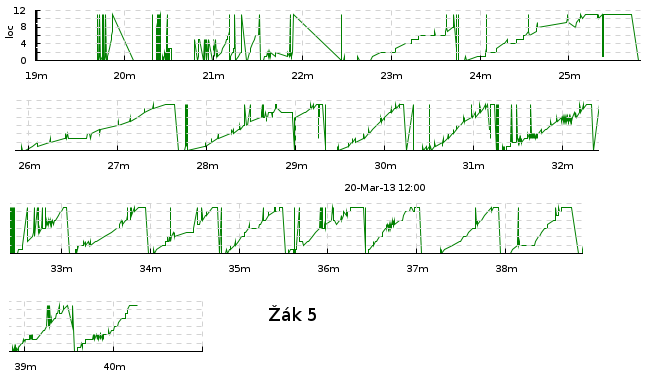
\includegraphics[width=1\textwidth]{Location5-cut}
\subsection{Žák 6}
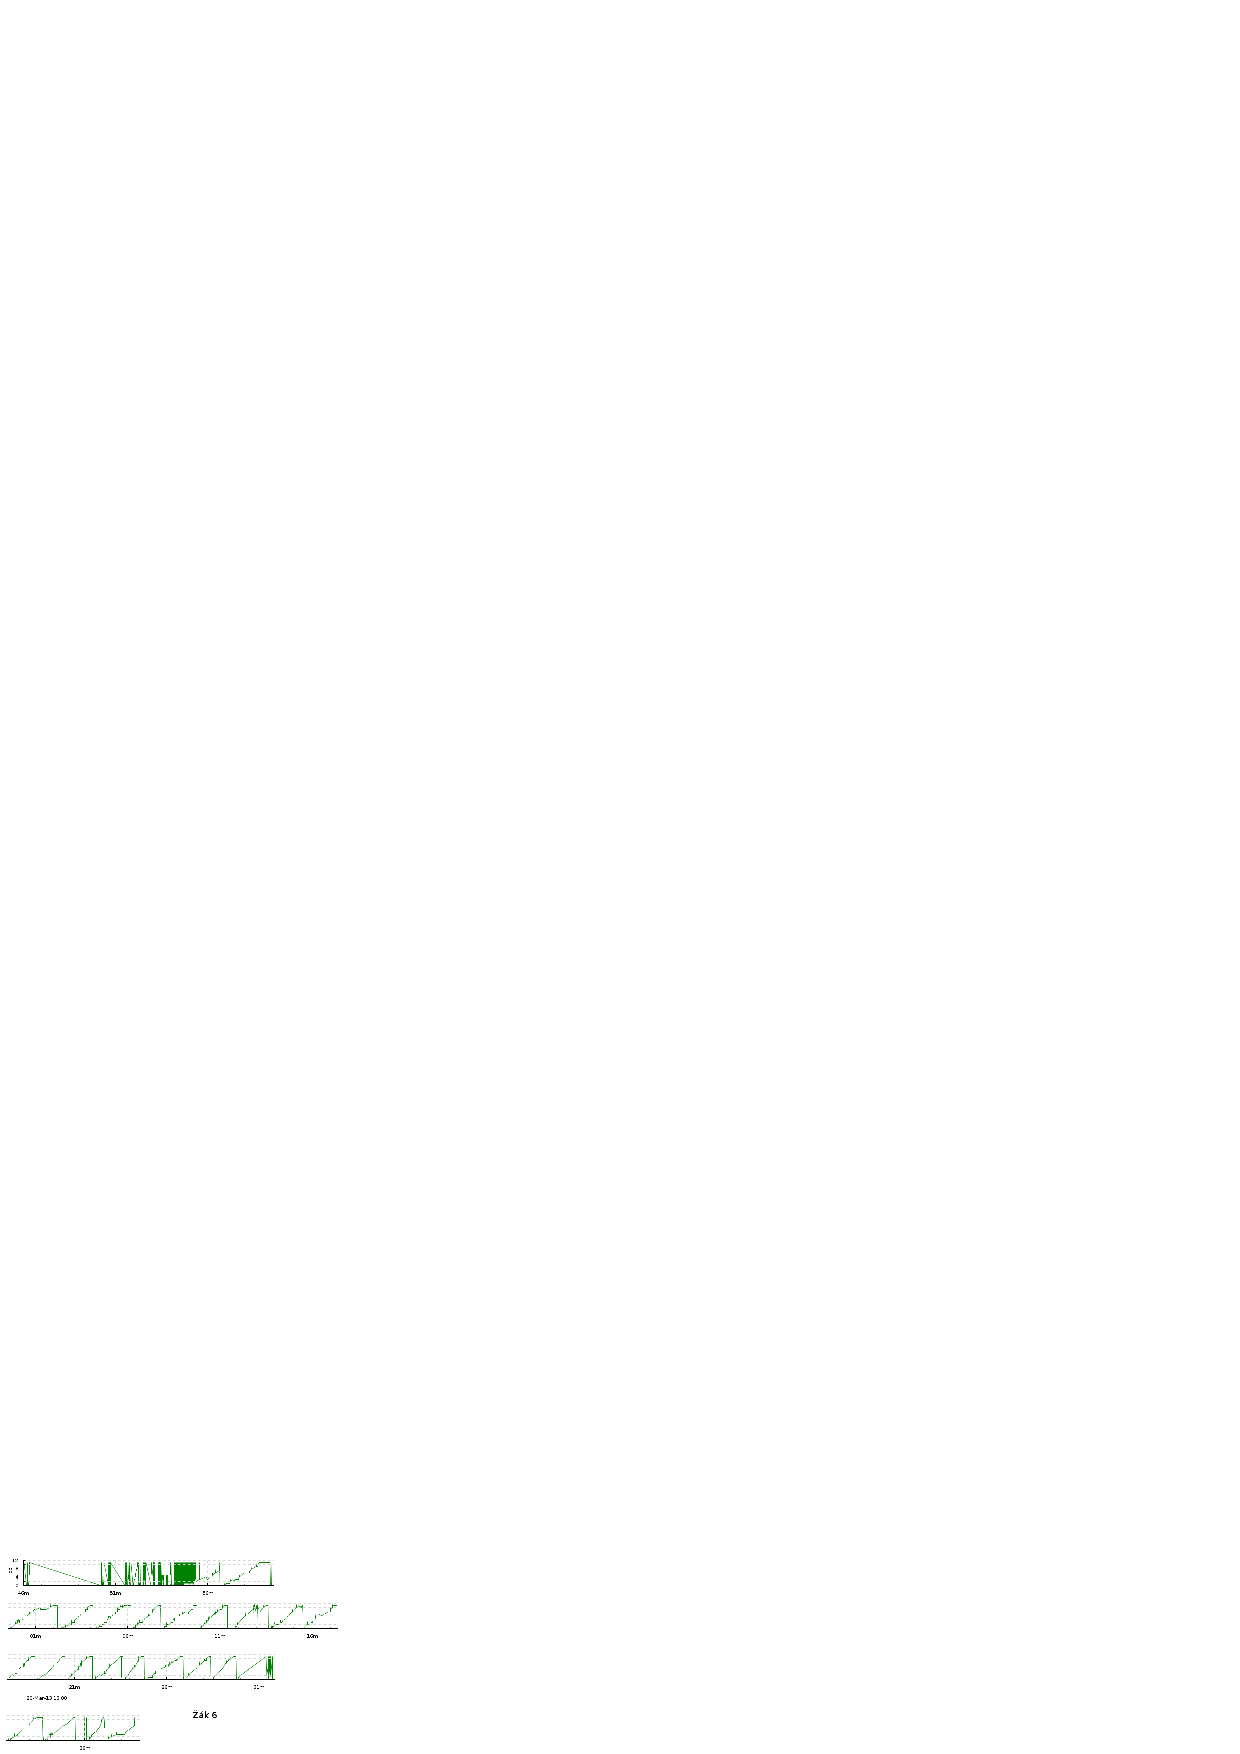
\includegraphics[width=1\textwidth]{Location6-cut}
\subsection{Žák 7}
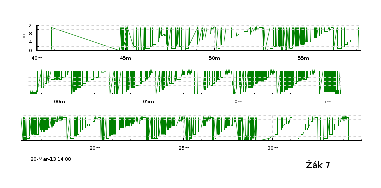
\includegraphics[width=1\textwidth]{Location7-cut}
\subsection{Žák 9}
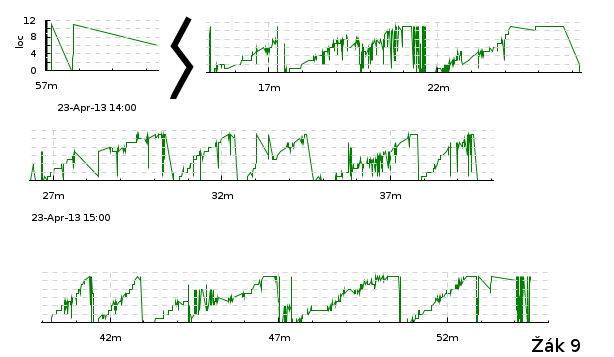
\includegraphics[width=1\textwidth]{Location9-cut}

\subsection{Analýza chyb}

Tady jsou shromážděné chyby účastníků běžného studie.  Zase neuvedu tady výsledky osmi účastníka.

\begin{tabular}{|c|c|}
\hline
Symbol&Význam\\
\hline
NČ&Nečetl samostatně\\
\hline
??&Chyba, ale nebyla poznat jaký na nahrávce\\
\hline
>>&Přeskočil písmeno\\
\hline
*&Není poznat jestli byly chyby kvůli vádám audiu\\
\hline
!&Znak pro velké písmena\\
\hline
--&Četl s pomoci\\
\hline
\end{tabular}


%\paragraph{První Řádek}
\begin{tabular}{|c|c|c|c|c|c|c|c|c|c|c|c|c|}
\hline
Žák&B&r&a&i&l&l&s&&&&&\\
&\braillebox{1278}&\braillebox{1235}&\braillebox{1}&\braillebox{24}&\braillebox{123}&\braillebox{123}&\braillebox{234}&\braillebox{}&\braillebox{2358}&\braillebox{123}&\braillebox{}&\braillebox{}\\
\hline
5&&&&\braillebox{234}&&&&&&&&\\
5&&NČ&NČ&s&&&&&&&&\\
\hline
6&\braillebox{1236}&&&&&&&&&&&\\
6&v&&&&??&&&&&&&\\
\hline
7&\braillebox{126}&\braillebox{125}&&\braillebox{2}&&&&&&&&\\
7&ě&h&&,&&>>&&&&&&\\
\hline
9&&&&&&&\braillebox{1234}&&&&&\\
9&NČ&--&&&&&p&&&&&\\
\hline
\end{tabular}

%\paragraph{Druhý Řádek}
\begin{tabular}{|c|c|c|c|c|c|c|c|c|c|c|c|c|}
\hline
Žák&k&ý& &ř&á&d&e&k&,& &k&t\\
&\braillebox{1378}&\braillebox{12346}&\braillebox{}&\braillebox{2456}&\braillebox{16}&\braillebox{145}&\braillebox{15}&\braillebox{13}&\braillebox{2}&\braillebox{}&\braillebox{13}&\braillebox{2345}\\
\hline
5&&&&&&&&&NČ&&&\\
\hline
6&\braillebox{1}&\braillebox{1234}&&\braillebox{2345}&&&&&&&&\braillebox{245}\\
6&a&?p?&&?t?&&&??&&NČ&&&j\\
\hline
7&&&&&&&&&&&&\\
\hline
9&&&&&&&&&&&&\braillebox{1}\\
9&&&&&&&&&&&&a\\
\hline
\end{tabular}

%\paragraph{Třetí Řádek}
\begin{tabular}{|c|c|c|c|c|c|c|c|c|c|c|c|c|}
\hline
Žák&e&r&ý& &t&e&ď& &p&o&u&ž\\
&\braillebox{1578}&\braillebox{1235}&\braillebox{12346}&\braillebox{}&\braillebox{2345}&\braillebox{15}&\braillebox{1456}&\braillebox{}&\braillebox{1234}&\braillebox{135}&\braillebox{136}&\braillebox{2346}\\
\hline
5&&&&&&??&&&&&&\\
\hline
6&&&&&&&&&&\braillebox{1235}&&\\
6&&&&&&&&&&r&&\\
\hline
7&&&&&&\braillebox{135}&&&&\braillebox{13}&&\\
7&&&&&&o&&&&k&&\\
\hline
9&&&&&&&&&&&&\braillebox{1356}\\
9&&&&&&&&&&&&z\\
\hline
\end{tabular}

%\paragraph{Čtvrtý Řádek}
\begin{tabular}{|c|c|c|c|c|c|c|c|c|c|c|c|c|}
\hline
Žák&í&v&á&t&e&,& &n&e&n&í& \\
&\braillebox{3478}&\braillebox{1236}&\braillebox{16}&\braillebox{2345}&\braillebox{15}&\braillebox{2}&\braillebox{}&\braillebox{1345}&\braillebox{15}&\braillebox{2345}&\braillebox{34}&\braillebox{}\\
\hline
5&&&&\braillebox{245}&&&&\braillebox{145}&&&&\\
5&&&&j&&&&d&&&&\\
\hline
6&&\braillebox{123}&&&&&&&&&&\\
6&&l&&&&&&&&&&\\
\hline
7&&&\braillebox{136}&&\braillebox{135}&&&\braillebox{145}&&&&\\
7&&&u&&o&&&d&&&&\\
\hline
9&\braillebox{16}&&&&\braillebox{24}&&&\braillebox{2346}&&&\braillebox{2345},\braillebox{16}&\\
9&á&&&&i&&&ž(NČ)&>>&>>&t,á&\\
\hline
\end{tabular}

%\paragraph{Pátý Řádek}
\begin{tabular}{|c|c|c|c|c|c|c|c|c|c|c|c|c|}
\hline
Žák&p&r&v&n&í& &ř&á&d&e&k&,\\
&\braillebox{123478}&\braillebox{1235}&\braillebox{1236}&\braillebox{1345}&\braillebox{34}&\braillebox{}&\braillebox{1235}&\braillebox{16}&\braillebox{145}&\braillebox{15}&\braillebox{13}&\braillebox{2}\\
\hline
5&&&&&&&&&&&&\\
\hline
6&&&&&&&&&&&\braillebox{1}&\\
6&&&&&&&&&&&a&NČ\\
\hline
7&&&&&&*&*&*&*&*&*&*\\
\hline
9&&&&&&&&\braillebox{34}&&&\braillebox{1}&\\
9&&&&&&&&í&&&a&\\
\hline
\end{tabular}

%\paragraph{Šestý Řádek}
\begin{tabular}{|c|c|c|c|c|c|c|c|c|c|c|c|c|}
\hline
Žák& &k&t&e&r&ý& &z&o&b&r&a\\
&\braillebox{78}&\braillebox{13}&\braillebox{2345}&\braillebox{15}&\braillebox{1235}&\braillebox{12346}&\braillebox{}&\braillebox{1356}&\braillebox{135}&\braillebox{12}&\braillebox{1235}&\braillebox{1}\\
\hline
5&&&&&&&&&&&&\\
\hline
6&&&&&&&&&&&&\\
\hline
7&&&&&&&&\braillebox{2456}&&&&\\
7&&&&&&&&ř&&&&\\
\hline
9&&&&&&&&\braillebox{1345}&&&\braillebox{125}&\\
9&&&&&&&&n&&&h&\\
\hline
\end{tabular}

%\paragraph{Řádek 7}
\begin{tabular}{|c|c|c|c|c|c|c|c|c|c|c|c|c|}
\hline
Žák&z&u&j&e& &j&e&n&o&m& &j\\
&\braillebox{135678}&\braillebox{136}&\braillebox{245}&\braillebox{15}&\braillebox{}&\braillebox{245}&\braillebox{15}&\braillebox{1345}&\braillebox{135}&\braillebox{134}&\braillebox{}&\braillebox{245}\\
\hline
5&&&&&&&&&&&&\\
\hline
6&&&&&&&&\braillebox{145}&&&&\\
6&&&&&&&&d&&&&\\
\hline
7&&&&&&&&&&&&\\
\hline
9&\braillebox{1345}&\braillebox{1}&\braillebox{125}&&&\braillebox{125}&&\braillebox{145}&&\braillebox{13}&&,\\
9&n&a&h&&&h&&d&&k&&,\\
\hline
\end{tabular}

%\paragraph{Řádek 8}
\begin{tabular}{|c|c|c|c|c|c|c|c|c|c|c|c|c|}
\hline
Žák&e&d&n&o& &p&í&s&m&e&n&o\\
&\braillebox{1578}&\braillebox{145}&\braillebox{1345}&\braillebox{135}&\braillebox{}&\braillebox{1234}&\braillebox{24}&\braillebox{234}&\braillebox{134}&\braillebox{15}&\braillebox{1345}&\braillebox{135}\\
\hline
5&&&&&&&&&&&&\\
\hline
6&&&&&&&&&&&&\\
\hline
7&&&&&&&&&&&&\braillebox{1}\\
7&&&&&&&&??&&&&a\\
\hline
9&&&&&&&\braillebox{16}&&\braillebox{14}&\braillebox{135}&&\braillebox{15}\\
9&&&&&&&á&&c&o&&e\\
\hline
\end{tabular}

%\paragraph{Řádek 9}
\begin{tabular}{|c|c|c|c|c|c|c|c|c|c|c|c|c|}
\hline
Žák&.& & &P&r&v&n&í& &b&y&l\\
&\braillebox{378}&\braillebox{}&\braillebox{}&\braillebox{12347}&\braillebox{1235}&\braillebox{1236}&\braillebox{1345}&\braillebox{34}&\braillebox{}&\braillebox{12}&\braillebox{13456}&\braillebox{123}\\
\hline
5&&&&&&&&&&&&\\
\hline
6&NČ&&&&&&&&&&&\\
\hline
7&&&&&&&&&&&&\\
\hline
9&\braillebox{236},\braillebox{6}&&&&&&&&&&&\\
9&(,!&&&&&&&&&&&\\
\hline
\end{tabular}

%\paragraph{Řádek 10}
\begin{tabular}{|c|c|c|c|c|c|c|c|c|c|c|c|c|}
\hline
Žák& &v&y&n&a&l&e&z&e&n& &v\\
&\braillebox{78}&\braillebox{1236}&\braillebox{13456}&\braillebox{1345}&\braillebox{1}&\braillebox{123}&\braillebox{15}&\braillebox{1356}&\braillebox{15}&\braillebox{1345}&\braillebox{}&\braillebox{1236}\\
\hline
5&&&&&&&&&&&&\\
\hline
6&&&\braillebox{1456}&&&&&&&&&\\
6&&&?ď ?&&&&&&&&&\\
\hline
7&&&&&&&\braillebox{135}&&&&&\\
7&&??&&&&&o&&&&&\\
\hline
9&&&&&&b&&&&&&\\
&&&&&&\braillebox{12}&&&&&&\\
\hline
\end{tabular}

%\paragraph{Řádek 11}
\begin{tabular}{|c|c|c|c|c|c|c|c|c|c|c|c|c|}
\hline
Žák& &r&o&c&e& &1&9&1&3& &v\\
&\braillebox{78}&\braillebox{1235}&\braillebox{135}&\braillebox{14}&\braillebox{15}&\braillebox{}&\braillebox{18}&\braillebox{248}&\braillebox{18}&\braillebox{148}&\braillebox{}&\braillebox{1236}\\
\hline
5&&&&&&&&&&&&\\
\hline
6&&&&&&&a&i&&&&\\
&&&&&&&\braillebox{1}&\braillebox{24}&&&&\\
\hline
7&&&&n&&&a&i&&&&l,r\\
&&&&\braillebox{1345}&&&\braillebox{1}&\braillebox{24}&&&&\braillebox{123},\braillebox{1235}\\
\hline
9&&ř&e,a&&&&a&i&&&&\\
&&\braillebox{2456}&\braillebox{15},\braillebox{1}&&&&\braillebox{1}&\braillebox{24}&&&&\\
\hline
\end{tabular}

%\paragraph{Řádek 12}
\begin{tabular}{|c|c|c|c|c|c|c|c|c|c|c|c|c|}
\hline
Žák& &A&n&g&l&i&i&.& & &J&m\\
&\braillebox{78}&\braillebox{17}&\braillebox{1345}&\braillebox{1245}&\braillebox{123}&\braillebox{24}&\braillebox{24}&\braillebox{3}&\braillebox{}&\braillebox{}&\braillebox{2457}&\braillebox{134}\\
\hline
5&&&d&&&&&mezera&&&&\\
&&&\braillebox{145}&&&&&\braillebox{}&&&&\\
\hline
6&&&&&&&9&&&&--&\\
&&&&&&&\braillebox{248}&&&&&\\
\hline
7&&&&&&e&&&&&&\\
&&&&&&\braillebox{15}&&&&&&\\
\hline
9&&&d&x&b&&&&&&,&c\\
&&&\braillebox{145}&\braillebox{1346}&\braillebox{12}&&&&&&\braillebox{2}&\braillebox{14}\\
\hline
\end{tabular}

%\paragraph{Řádek 13}
\begin{tabular}{|c|c|c|c|c|c|c|c|c|c|c|c|c|}
\hline
Žák&e&n&o&v&a&l& &s&e& &O&p\\
&\braillebox{1578}&\braillebox{1345}&\braillebox{135}&\braillebox{1236}&\braillebox{1}&\braillebox{123}&\braillebox{}&\braillebox{234}&\braillebox{15}&\braillebox{}&\braillebox{1357}&\braillebox{1234}\\
\hline
5&&&&&&&&&&&n&\\
&&&&&&&&&&&\braillebox{1345}&\\
\hline
6&*&*&r&&&&&&&&&\\
&&&\braillebox{1235}&&&&&&&&&\\
\hline
7&&&&l&&&&&&&&\\
&&&&\braillebox{123}&&&&&&&&\\
\hline
9&&&e&&&&&&&&k&l\\
&&&\braillebox{15}&&&&&&&&\braillebox{13}&\braillebox{123}\\
\hline
\end{tabular}

%\paragraph{Řádek 14}
\begin{tabular}{|c|c|c|c|c|c|c|c|c|c|c|c|c|}
\hline
Žák&t&o&f&o&n& &a& &p&ř&e&v\\
&\braillebox{234578}&\braillebox{135}&\braillebox{124}&\braillebox{135}&\braillebox{1345}&\braillebox{}&\braillebox{1}&\braillebox{}&\braillebox{1234}&\braillebox{2456}&\braillebox{15}&\braillebox{1236}\\
\hline
5&&&&&&&&&&&&\\
\hline
6&j&&&&&&&&n&&&\\
&\braillebox{245}&&&&&&&&\braillebox{1345}&&&\\
\hline
7&&&&&&&&&&&&\\
\hline
\end{tabular}

%\paragraph{Řádek 15}
\begin{tabular}{|c|c|c|c|c|c|c|c|c|c|c|c|c|}
\hline
Žák&á&d&ě&l& &s&v&ě&t&l&o& \\
&\braillebox{1678}&\braillebox{145}&\braillebox{126}&\braillebox{123}&\braillebox{}&\braillebox{234}&\braillebox{1236}&\braillebox{126}&\braillebox{2345}&\braillebox{123}&\braillebox{135}&\braillebox{}\\
\hline
5&&&&&&&&&&&&\\
\hline
6&&&v&&&i&&&j&&&\\
&&&\braillebox{1346}&&&\braillebox{15}&&&\braillebox{245}&&&\\
\hline
7&&&&&&&&&&&&\\
\hline
\end{tabular}

%\paragraph{Řádek 16}
\begin{tabular}{|c|c|c|c|c|c|c|c|c|c|c|c|c|}
\hline
Žák&n&a& &z&v&u&k&.& & &K&d\\
&\braillebox{134578}&\braillebox{1}&\braillebox{}&\braillebox{1356}&\braillebox{1236}&\braillebox{136}&\braillebox{13}&\braillebox{3}&\braillebox{}&\braillebox{}&\braillebox{137}&\braillebox{145}\\
\hline
5&&&&e&&&&&&&&\\
&&&&\braillebox{15}&&&&&&&&\\
\hline
6&&&&&&&&&&&&\\
\hline
7&&&&&&&&&&&&\\
\hline
\end{tabular}

%\paragraph{Řádek 17}
\begin{tabular}{|c|c|c|c|c|c|c|c|c|c|c|c|c|}
\hline
Žák&y&ž& &č&t&e&n&á&ř& &p&o\\
&\braillebox{1345678}&\braillebox{2346}&\braillebox{}&\braillebox{146}&\braillebox{2345}&\braillebox{15}&\braillebox{1345}&\braillebox{16}&\braillebox{2456}&\braillebox{}&\braillebox{1234}&\braillebox{135}\\
\hline
5&&&&&&&&&&&&\\
\hline
6&&&&&j&&k&&&&&\\
&&&&&\braillebox{245}&&\braillebox{13}&&&&&\\
\hline
7&ď&&&??&&&&&&&&\\
&\braillebox{1456}&&&&&&&&&&&\\
\hline
\end{tabular}

%\paragraph{Řádek 18}
\begin{tabular}{|c|c|c|c|c|c|c|c|c|c|c|c|c|}
\hline
Žák&h&y&b&o&v&a&l& &s&p&e&c\\
&\braillebox{12578}&\braillebox{13456}&\braillebox{12}&\braillebox{135}&\braillebox{1236}&\braillebox{1}&\braillebox{123}&\braillebox{}&\braillebox{234}&\braillebox{1234}&\braillebox{15}&\braillebox{14}\\
\hline
6&&&&&&&&&&&&\\
\hline
7&??&d&&&&&&&&&&\\
&&\braillebox{145}&&&&&&&&&&\\
\hline
\end{tabular}

%\paragraph{Řádek 19}
\begin{tabular}{|c|c|c|c|c|c|c|c|c|c|c|c|c|}
\hline
Žák&i&á&l&n&í&m& &p&e&r&e&m\\
&\braillebox{2478}&\braillebox{16}&\braillebox{123}&\braillebox{1345}&\braillebox{34}&\braillebox{134}&\braillebox{}&\braillebox{1234}&\braillebox{15}&\braillebox{1235}&\braillebox{15}&\braillebox{134}\\
\hline
6&&&&&&&&&&&&\\
\hline
7&s&e&&&&&&&o&&&p\\
7&\braillebox{234}&\braillebox{15}&&&&&&&\braillebox{135}&&&\braillebox{1234}\\
\hline
\end{tabular}

%\paragraph{Řádek 20}
\begin{tabular}{|c|c|c|c|c|c|c|c|c|c|c|c|c|}
\hline
Žák& &n&a&d& &p&í&s&m&e&n&e\\
&\braillebox{78}&\braillebox{1345}&\braillebox{1}&\braillebox{145}&\braillebox{}&\braillebox{1234}&\braillebox{34}&\braillebox{234}&\braillebox{134}&\braillebox{15}&\braillebox{1345}&\braillebox{15}\\
\hline
6&&&&&&&&&&&&\\
\hline
\end{tabular}

%\paragraph{Řádek 21}
\begin{tabular}{|c|c|c|c|c|c|c|c|c|c|c|c|c|}
\hline
Žák&m&,& &p&ř&í&s&t&r&o&j& \\
&\braillebox{13478}&\braillebox{2}&\braillebox{}&\braillebox{1234}&\braillebox{2456}&\braillebox{34}&\braillebox{234}&\braillebox{2345}&\braillebox{1235}&\braillebox{135}&\braillebox{245}&\braillebox{}\\
\hline
6&&&&&&&&&&&&\\
\hline
\end{tabular}

%\paragraph{Řádek 22}
\begin{tabular}{|c|c|c|c|c|c|c|c|c|c|c|c|c|}
\hline
Žák&b&z&u&č&e&l&.& & &T&o& \\
&\braillebox{1278}&\braillebox{1356}&\braillebox{136}&\braillebox{146}&\braillebox{15}&\braillebox{123}&\braillebox{3}&\braillebox{}&\braillebox{}&\braillebox{23457}&\braillebox{135}&\braillebox{}\\
\hline
6&&&&&&&&&&&&\\
\hline
\end{tabular}

\section{Analýza a srovnání s podobnými studii}

\subsection{Swift}
Vrátíme-li k Swiftův rozdělení druhů učení vidíme, že moje studie obsahovala všechní tři druhu.  Účastnicí získali dovednost používat selektor.  Účastnicí trénovali souvislost mezi mezi malé Braillovo písmo, které již znají a velké Braillovo, které se zobrazuje na zobrazovače FCHADu.  Účastnicí odvykli od toho používat selektor jako piezoelektrický braillský řádek a tím pádem trénování inhibice.

\subsection{Anderson}
\subsection{Vlastní model}
Je možný, že to, jak žáci často nemohli říct, který písmo je "Jedná, dva, tři, pět" byla moje chyba jako pedagog jsem nesprávně odhadl před znalost.
\subsection{Optacon}
\subsection{Patterson a Lee}
